\documentclass[11pt]{article}
\usepackage[a4paper,margin=1in]{geometry}
\usepackage{amsmath,amssymb,amsthm,mathtools}
\usepackage[expansion=false]{microtype}
\usepackage{graphicx,booktabs,array}
\usepackage[font=small,labelfont=bf]{caption}
\usepackage[dvipsnames]{xcolor}
\usepackage{enumitem}
\usepackage[hidelinks,pdfusetitle]{hyperref}
\usepackage[nameinlink,capitalise]{cleveref}
\setlist{nosep,leftmargin=1.5em}
\newtheorem{theorem}{Theorem}[section]
\newtheorem{lemma}[theorem]{Lemma}
\newtheorem{proposition}[theorem]{Proposition}
\newtheorem{corollary}[theorem]{Corollary}
\newtheorem{principle}{Principle}
\theoremstyle{definition}\newtheorem{definition}[theorem]{Definition}
\theoremstyle{remark}\newtheorem{remark}[theorem]{Remark}
\newcommand{\Z}{\mathbb Z}\newcommand{\N}{\mathbb N}
\newcommand{\dd}{\,\mathrm d}\newcommand{\e}{\mathrm e}
\DeclareMathOperator{\Li}{Li}
\setlength{\parskip}{0.35em}
\AtBeginDocument{\sloppy}
\urlstyle{same}
\hypersetup{pdftitle={Nothing Binds a Twin but Exclusion},pdfauthor={Abhijit Singh}}
\title{\textbf{Nothing Binds a Twin but Exclusion}\\[6pt]
\large The Prime Clocks, the Exclusion Law, and the Recurrence of the Twin Pair}
\author{Abhijit Singh}
\date{}
\begin{document}
\maketitle

\begin{abstract}
We read the integers prime to $6$ as the positions of a world of clocks. Each prime $p\ge5$ is a clock that marks the two centres $k$ with $6k\equiv\pm1\pmod p$, and a centre that no clock marks is a \emph{full zero}; below the reach of the clocks a full zero is exactly a twin prime pair $6k\pm1$. We prove what the step from one clock to the next preserves: the full zeros per turn number $\prod(p-2)$, the pattern is a palindrome, the new world is made of $P'-2$ exact copies of the old one, and the copy sign sums to $\prod(p-4)>0$. We then prove that the two members of a pair are bound by exactly one relation: \emph{a clock may mark one member, and then it does not mark the other.} Everything else about the pair is the product of its two single members. We call this the \emph{exclusion law}. It fixes the twin constant as the exclusion product $E=\prod_{p\ge5}\bigl(1-(p-1)^{-2}\bigr)=0.88022\ldots$, and with the density $3/\log x$ of primes among the numbers $6k\pm1$ it gives the twin law
\[
\pi_2(x)\sim\frac x6\Bigl(\frac3{\log x}\Bigr)^{2}E=\frac{2C_2\,x}{\log^2x}.
\]
We state as a principle what the construction implies: independence is the absence of a relation, and a relation needs a clock. Under this principle the twin pair recurs at every level of the clocks, and there are infinitely many twin primes. Every measurement agrees with the exclusion law and with nothing beyond it. The joint law of the number of prime factors of $6k-1$ and $6k+1$, taken over $5\cdot10^7$ pairs, gives the prime--prime factor $0.8833$ against $E=0.8802$. The pair symbol $\sum z^{\Omega(6k-1)}w^{\Omega(6k+1)}$ factorises to the same constant. On the frame of rough pairs the share of twins equals the product of the members' shares to within $1\%$. The count of twin pairs up to $10^{10}$, $27{,}412{,}679$, is the law to within $5$ parts in $10^5$. We prove that twins are forced wherever the primes are the majority of rough numbers, which is the case for $u=\log y/\log z<3.565$. In the reach of the clocks, where $u=2$, the bound is an equality, twins $=U$. There each member keeps $\e^\gamma\omega(2)=\e^\gamma/2$ of its share over a turn, which is a theorem. The twin pairs keep the product of the two members' factors to within $0.3\%$ at $P=31601$, so the size of $U$ there is the twin law itself. We show that the parity barrier of sieve theory is a ceiling of the instrument, not a property of the primes: information about the distribution of primes in progressions certifies at most $48.837\%$ of the rough members as prime, and every frame reaches the required $100\%$ only in the degenerate limit where the inequality reads \emph{twins $\ge$ twins}. The same reading organises single primes and central values. A single number is its own copy exactly $\lfloor\sqrt x\rfloor$ times, $\sum_{n\le x}\lambda(n)\lfloor x/n\rfloor=\lfloor\sqrt x\rfloor$, while a pair never is. Prime squares sit only on the $+$ side of the triad, and the class lean of prime pairs lives only on the member on that side. For $17$ $L$-functions the lean of the primes equals $-\nu/2-r$, with $\nu$ the self-copy count and $r$ the order of the central zero. The central value of the congruent-number curve $y^2=x^3-n^2x$ is $4\kappa_n m^2$ with $m\in\Z$, so it is either $0$ or at least $4\kappa_n/\sqrt n$.
\end{abstract}

\tableofcontents

%======================================================================
\section{Introduction: what binds a twin}\label{sec:intro}

Two odd numbers $6k-1$ and $6k+1$ share one thing, their centre $6k$, and differ by $2$. The twin prime question asks whether infinitely often both are prime. This paper asks a prior question: \emph{what binds the two members of a pair?} If nothing binds them except what the construction of the integers visibly puts between them, then the twin pair must recur exactly as often as two unbound members would both be prime, corrected by that one visible bond. The work of the paper is to find the bond, to prove that it is the only one, and to measure the pair against it.

The bond is found in \cref{sec:exclusion}. Each prime $p\ge5$ acts on the centres as a clock with two marks, one for each member. The two marks are different classes modulo $p$, so a prime can divide one member or the other but never both. This \emph{exclusion} is the whole of the relation. In the world of clocks it is a theorem that everything else about the pair is the product of its single members (\cref{thm:exclusion}). The exclusion changes the product by the factor $1-(p-1)^{-2}$ at each clock, and their product is the twin constant.

The measurements of \cref{sec:measure,sec:law} test the pair against the bond and find nothing beyond it: not in the joint law of the prime factors of the two members, not in the generating symbol of that law at any radius, not on the frame of rough pairs, and not in the count of twin pairs to $10^{10}$.

\Cref{sec:instrument} addresses the reason the question has been held to be closed to the methods that prove the most about primes. It shows that the obstruction, known as the parity barrier, is a ceiling of an instrument. The instrument is information about how primes are spread over residue classes. It cannot tell a prime from a product of two large primes, and when that is measured exactly it certifies $48.837\%$ where a majority is needed. That ceiling describes the instrument. It says nothing about whether the members of a pair are bound.

\Cref{sec:self-copy,sec:centre} show that the same reading, a thing and its copy, a pair and its mirror, organises the lean of single primes, the rank of elliptic curves at the centre, and the central value of the congruent-number curves. \Cref{sec:whole} records, for each problem, which of its claims the generating step returns whole.

\paragraph{Main results.} In one line each:
\begin{enumerate}[label=(\roman*)]
\item The step from the clocks up to $P$ to the clocks up to $P'$ builds the new world from $P'-2$ exact copies of the old one (\cref{thm:copies}). The count $\prod(p-2)$, the palindrome and the copy sign $\prod(p-4)>0$ are preserved (\cref{thm:count,thm:marking}).
\item The two members of a pair are related only by exclusion at each clock; everything else is the product of the members (\cref{thm:exclusion}).
\item Under the principle that independence is the absence of a relation (\cref{pr:independence}), the twin law holds and the twin pair recurs at every level (\cref{thm:law}).
\item Twins are forced by majority wherever primes outnumber the other rough numbers (\cref{thm:pigeonhole}). Distribution information certifies at most $48.837\%$ (\cref{prop:ceiling}). In the reach of the clocks, $u=2$, the bound is the equality twins $=U$, and each member keeps $\e^\gamma/2$ of its share over a turn (\cref{prop:window}).
\item A single is its own copy $\lfloor\sqrt x\rfloor$ times; a pair never is (\cref{thm:copy}). The squares sit on the $+$ side, and so does the lean of prime pairs (\cref{thm:side,prop:lean}).
\item The central value of the congruent-number curve is $4\kappa_n m^2$ with $m\in\Z$ (\cref{thm:square}).
\end{enumerate}

%======================================================================
\section{The world of clocks}\label{sec:clocks}

\begin{definition}[centres, clocks, full zeros]\label{def:clocks}
A \emph{centre} is an integer $k$. It carries the pair $(6k-1,6k+1)$, the \emph{lower} and \emph{upper} member. For a prime $p\ge5$ let $r_p\equiv6^{-1}\pmod p$. The \emph{clock} $p$ marks the centres
\[
M_p=\{k:\ k\equiv r_p\ \text{or}\ k\equiv-r_p\pmod p\}=\{k:\ p\mid(6k-1)(6k+1)\}.
\]
At \emph{level} $P$ the full zeros are $Z_P=\{k:\ k\notin M_p\ \text{for all primes}\ 5\le p\le P\}$. The pattern is periodic with period, the \emph{turn}, $Q_P=\prod_{5\le p\le P}p$.
\end{definition}

The two marks of a clock are $r_p$ and $-r_p$; they differ by $2r_p\equiv3^{-1}$, a third of the turn of the clock. The mark $k\equiv r_p$ is the lower member divisible by $p$, and $k\equiv-r_p$ the upper.

\begin{figure}[t]\centering
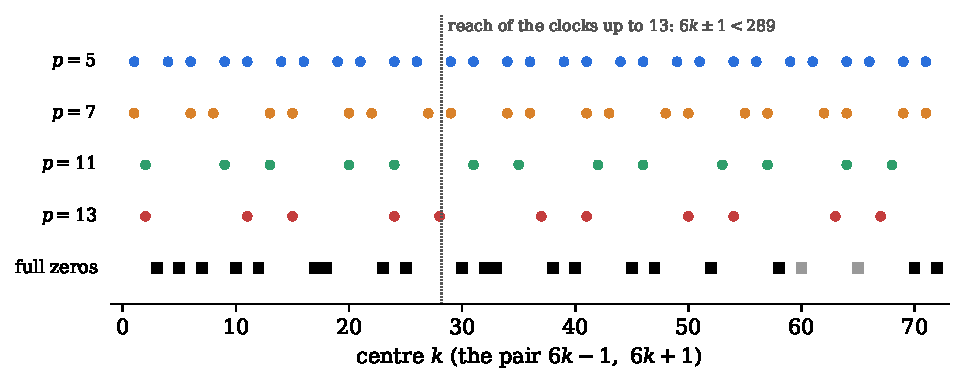
\includegraphics[width=\linewidth]{fig1_clocks.pdf}
\caption{The clocks $5,7,11,13$ over the centres $0\le k\le72$. Each clock marks two centres per turn, one for each member of the pair. Black squares are the full zeros that are twin primes. Grey squares are full zeros beyond the reach of these clocks, where a member may be a product of two primes above $13$. Left of the dotted line every full zero is a twin prime pair.}
\label{fig:clocks}
\end{figure}

\begin{proposition}[the mirror window is the twin question]\label{prop:mirror}
Let $P<P'$ be consecutive primes and $k\ge1$ with $6k-1>P$ and $6k+1<P'^2$. Then $k\in Z_P$ if and only if $6k-1$ and $6k+1$ are both prime.
\end{proposition}
\begin{proof}
A number below $P'^2$ that is prime to $6$ and to every prime up to $P$ has no prime factor below $P'$, so it is $1$ or a prime.
\end{proof}

The \emph{reach} of the clocks up to $P$ is therefore the range of centres $6k+1<P'^2$. The window of centres around $0$ is the \emph{mirror window}: it is where the actual primes live. Every other window of a turn is a rotation of the clocks, in which a full zero is a pair of numbers free of small factors but not necessarily prime (\cref{fig:mirror}).

%======================================================================
\section{What the step preserves}\label{sec:step}

\begin{theorem}[count and palindrome]\label{thm:count}
In each turn of level $P$ there are exactly $\prod_{5\le p\le P}(p-2)$ full zeros, and $Z_P=-Z_P$.
\end{theorem}
\begin{proof}
Going from $P$ to the next prime $P'$, each full zero $k$ of a turn of level $P$ lifts to the $P'$ centres $k+jQ_P$, $0\le j<P'$. These have distinct residues modulo $P'$, because $Q_P$ is prime to $P'$, so exactly two of them are marked by the new clock. Hence $|Z_{P'}|=(P'-2)|Z_P|$ per turn. The marks $\pm r_p$ are symmetric under $k\mapsto-k$, so each level is a palindrome.
\end{proof}

\begin{theorem}[the step builds the world from copies of itself]\label{thm:copies}
Let $P<P'$ be consecutive primes and $c$ a residue class modulo $P'$. If $c\equiv\pm r_{P'}$, the class contains no full zero of level $P'$. Otherwise
\[
\{j\in\Z:\ c+P'j\in Z_{P'}\}=\{j\in\Z:\ c+P'j\in Z_P\},
\]
which is the full-zero set of level $P$ read along the affine map $j\mapsto c+P'j$: a copy of level $P$ with the same count per turn, symmetric about its own centre.
\end{theorem}
\begin{proof}
The clock $P'$ marks exactly the classes $\pm r_{P'}$. On every other class it marks nothing, so a centre $c+P'j$ is a full zero of level $P'$ if and only if it is one of level $P$. Since $P'$ is invertible modulo $Q_P$, the map $j\mapsto c+P'j$ runs once through all residues modulo $Q_P$ in a period, which gives the count.
\end{proof}

The new world is made of the old one: $P'-2$ copies and two empty classes (\cref{fig:copies}). This is the precise sense in which the pattern at every level is the same simple rule recurring. The step also preserves the full distribution of marks.

\begin{figure}[t]\centering
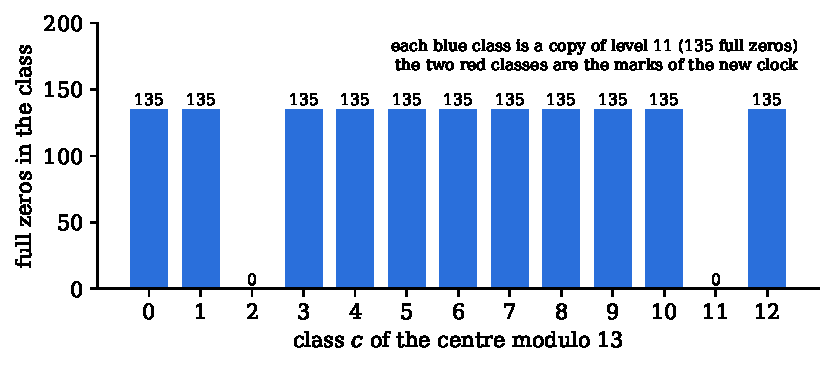
\includegraphics[width=0.78\linewidth]{fig2_copies.pdf}
\caption{Level $13$ read class by class modulo $13$. Eleven classes are exact copies of level $11$, each with $135$ full zeros. The two classes $\pm r_{13}$ are the marks of the new clock and are empty. The same holds exactly for $13\to17$ ($1485$ per class) and $17\to19$ ($22275$ per class).}
\label{fig:copies}
\end{figure}

\begin{theorem}[marking law and copy sign]\label{thm:marking}
In a turn of level $P$, the number of centres marked by exactly $j$ clocks is the coefficient of $x^j$ in $\prod_{5\le p\le P}\bigl((p-2)+2x\bigr)$. In particular the copy sign $(-1)^{\#\text{clocks marking }k}$ sums over a turn to $\prod_{5\le p\le P}(p-4)>0$.
\end{theorem}
\begin{proof}
In the lifting of \cref{thm:count}, each centre lifts to $p-2$ centres that the new clock leaves unmarked and $2$ that it marks. Set $x=-1$ for the sign.
\end{proof}

Both identities were checked exactly over full turns for $P=7,11,13,17,19$ (sign sums $3,21,189,2457,36855$).

\paragraph{Windows do not return whole.} Inside each copy of \cref{thm:copies}, a window of $L$ consecutive centres of level $P'$ appears as a window of length about $L/P'$. A statement of the form ``every window of length $L_P$ holds a full zero'' therefore passes from level $P$ to level $P'$ only if $L_{P'}\le P'L_P$. The reach grows like $P^2$ while the copies grow like $P$, so window statements about the reach never return whole under the step: each application hands the question to a shorter window one modulus deeper. The step returns whole the counts over a turn, not the windows.

The strongest window statement, that the longest run $H(P)$ of centres without a full zero is shorter than the reach, has been computed exactly for all rotations of the clocks up to $41$ (\cref{tab:holes}). Asked of all rotations, it is at least as demanding as a two-class form of Jacobsthal's problem. For one class, the best proved bound is still of the order of the square of the largest clock \cite{Iwaniec78}, and the longest runs are known to exceed the average spacing by more than a logarithm \cite{FGKMT}. The twin question asks for much less: it concerns only the mirror window. That window is not a worst case. At $P=23$ it holds $35$ full zeros, against a mean of $28.87$ and a maximum of $39$ over the $37{,}182{,}145$ windows of the turn (\cref{fig:mirror}).

\begin{remark}[window statistics over a turn]\label{rem:variance}
Over a full turn, the joint law of two full zeros at distance $h$ is exact: $\rho_2(h)=\prod_p(p-c_p(h))/p$, where $c_p=2$ if $p\mid h$, $c_p=3$ if $3h\equiv\pm1\pmod p$, and $c_p=4$ otherwise. This gives the variance of the number of full zeros in a window exactly. It is $3.781$ at $P=19$ and $5.157$ at $P=23$, against the enumerated $3.76$ and $5.15$. The ratio of variance to mean is $0.18$ to $0.32$ for $P\le1601$, so full zeros are three to five times more evenly spread than independent points. The counts are Gaussian over the turn, and their lower tail is thinner than the Gaussian at the exact variance. Compare the singular-series variance of primes in short intervals \cite{Gallagher76,MS04}. Brun's method, subtracting the marks clock by clock, certifies a full zero in every window only up to a length $P^{e(P)}$, with $e(P)=4.17$ at $P=29$ and $8.94$ at $P=10^6$ \cite{Brun19}. The dimension-two sieve \cite{DH08} is the refined form of the same instrument.
\end{remark}

\begin{table}[t]\centering\small
\begin{tabular}{@{}lccccccccc@{}}\toprule
$P$ & 11&13&17&19&23&29&31&37&41\\\midrule
longest run $H(P)$ & 6&10&17&24&33&42&57&87&90\\
reach $(P^2-P)/6$ & 18.3&26&45.3&57&84.3&135.3&155&222&273.3\\\bottomrule
\end{tabular}
\caption{Exact longest runs over all rotations of the clocks up to $P$, against the reach. The ratio stays between $0.31$ and $0.42$. Following only the sparsest windows from level to level reproduces $H(P)$ exactly up to $P=37$. At $41$ the longest run comes from a window that was not among the sparsest at the lower levels.}
\label{tab:holes}
\end{table}

\begin{figure}[t]\centering
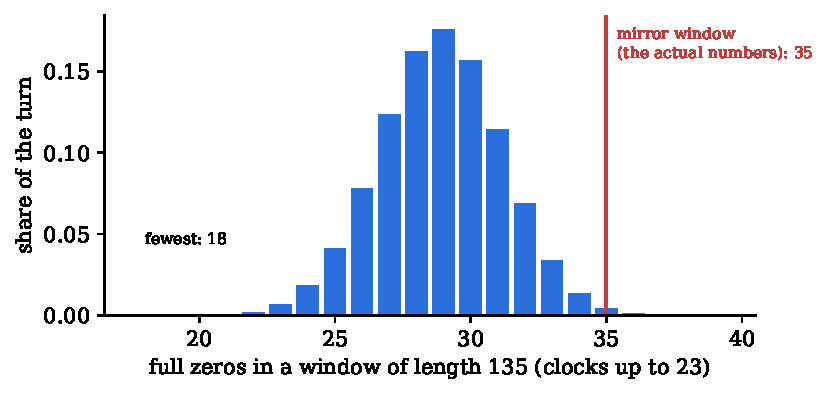
\includegraphics[width=0.78\linewidth]{fig8_mirror.pdf}
\caption{Full zeros in all windows of $135$ centres over a turn of the clocks up to $23$. The mirror window, the one that contains the actual numbers, holds $35$, near the top of the distribution; the fewest in any rotation is $18$.}
\label{fig:mirror}
\end{figure}

%======================================================================
\section{The exclusion law}\label{sec:exclusion}

\begin{theorem}[exclusion law]\label{thm:exclusion}
Let $k$ be a uniformly chosen centre of a turn of level $P$. For each clock $p\le P$ let $X_p=1$ if $p\mid6k-1$ and $Y_p=1$ if $p\mid6k+1$, and $0$ otherwise. Then:
\begin{enumerate}[label=\textup{(\roman*)}]
\item the pairs $(X_p,Y_p)$ for different clocks are independent;
\item $\Pr(X_p=1)=\Pr(Y_p=1)=1/p$;
\item $\Pr(X_p=1,\,Y_p=1)=0$.
\end{enumerate}
The two members are bound only by \textup{(iii)}. In particular
\[
\Pr(k\in Z_P)=\prod_{5\le p\le P}\Bigl(1-\frac2p\Bigr)=\underbrace{\prod\Bigl(1-\frac1p\Bigr)}_{\text{lower member}}\ \underbrace{\prod\Bigl(1-\frac1p\Bigr)}_{\text{upper member}}\ \underbrace{\prod\Bigl(1-\frac1{(p-1)^2}\Bigr)}_{\text{exclusion}}.
\]
\end{theorem}
\begin{proof}
(i) is the Chinese remainder theorem over the turn. (ii) holds because each of the classes $\pm r_p$ is one class of $p$. (iii) holds because $r_p\not\equiv-r_p$ for $p\ge5$: no prime divides two numbers that differ by $2$. The factorisation is the identity $1-2/p=(1-1/p)^2\bigl(1-(p-1)^{-2}\bigr)$.
\end{proof}

\begin{corollary}[the twin constant is the exclusion product]\label{cor:constant}
The share of full zeros relative to the product of the members' survival shares tends, as $P\to\infty$, to
\[
E=\prod_{p\ge5}\Bigl(1-\frac1{(p-1)^2}\Bigr)=0.88021\ldots,\qquad \tfrac34E=C_2=\prod_{p\ge3}\Bigl(1-\frac1{(p-1)^2}\Bigr)=0.66016\ldots
\]
The factor $\tfrac34$ is the clock $3$, already absorbed by writing every pair as $6k\pm1$.
\end{corollary}

\Cref{thm:exclusion} is a complete list of relations. The only mechanism in the construction that ties one member to the other is a clock. A clock ties them in exactly one way, by taking one member and thereby leaving the other.

%======================================================================
\section{The pair measured against the exclusion law}\label{sec:measure}

\paragraph{The joint law of prime factors.} For the $5\cdot10^7$ centres with $6k+1\le3\cdot10^8$ let $N_{ab}$ count the centres with $\Omega(6k-1)=a$ and $\Omega(6k+1)=b$. Put $D_{ab}=N_{ab}K/(N_aN_b)$, where $K$ is the number of centres and $N_a,N_b$ are the marginal counts. If the members were unbound, every $D_{ab}$ would be $1$. \Cref{fig:exclusion} shows the table. The prime--prime entry is $D_{11}=0.8833$, against the exclusion product $E=0.8802$. The other entries show the smooth negative association that exclusion produces: a clock taken by one member cannot be taken by the other, so large factor counts avoid each other.

\begin{figure}[t]\centering
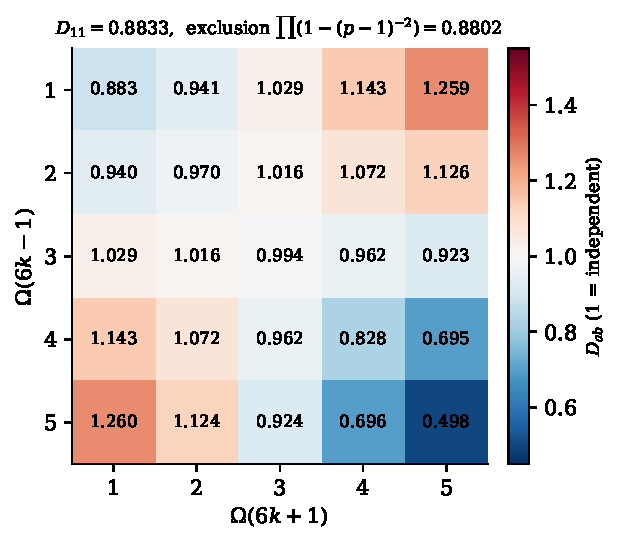
\includegraphics[width=0.52\linewidth]{fig3_exclusion.pdf}\hfill
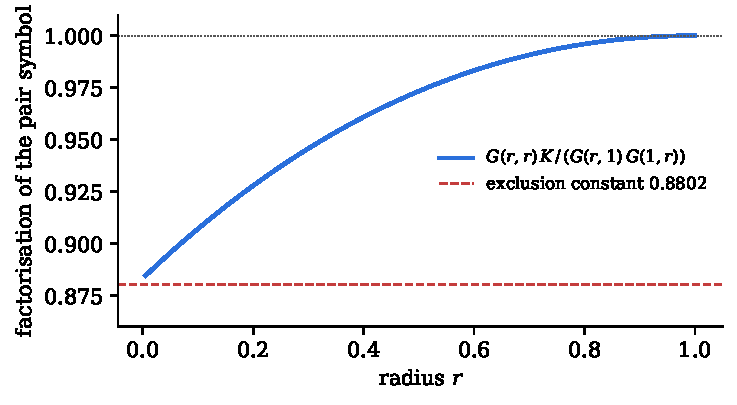
\includegraphics[width=0.46\linewidth]{fig4_symbol.pdf}
\caption{Left: the joint law of $\Omega(6k-1)$ and $\Omega(6k+1)$ relative to independence, over $5\cdot10^7$ pairs. The prime--prime entry equals the exclusion product to $0.3\%$. Right: the pair symbol $G(z,w)$ tested for factorisation on the circle $z=w=r$. As $r\to0$ the symbol isolates the prime--prime coefficient and the defect tends to the exclusion constant; at $r=1$ it is $1$.}
\label{fig:exclusion}
\end{figure}

\paragraph{The pair symbol.} Define
\[
G(z,w;x)=\sum_{6k+1\le x}z^{\Omega(6k-1)}\,w^{\Omega(6k+1)}.
\]
For fixed $z$ and $w$ with $|z|,|w|\le1$, the map $n\mapsto z^{\Omega(n)}$ is completely multiplicative and bounded. Exchanging $z$ and $w$ is the mirror of the pair. The number of twin centres is the single coefficient $[z^1w^1]G$, so ``the members are unbound'' is the statement that $G(z,w)$ factorises as $G(z,1)G(1,w)/K$ up to the exclusion. Measured on the circle $z=w=r$, the defect of factorisation is $0.973$ at $r=0.5$, $0.937$ at $0.25$, $0.907$ at $0.1$ and $0.888$ at $0.02$. As $r\to0$ it tends to the exclusion constant, as it must if exclusion is the only bond (\cref{fig:exclusion}).

\paragraph{The rough frame.} Fix $z$ and $y=z^u$. Call a pair \emph{rough} when both members are free of every prime up to $z$. On this frame each member is either prime or a product of primes above $z$, and \cref{thm:exclusion} has already been applied to every clock up to $z$. Let $R$ be the share of twins among rough pairs divided by the product of the prime shares of the two members. \Cref{tab:frame} and \cref{fig:frame} give $R$ for $z$ up to $1000$ and $y$ up to $10^9$. It is $1$ to within $1\%$ throughout: beyond the clocks already accounted for, the members decide their primality as two unbound numbers.

\begin{table}[t]\centering\small
\begin{tabular}{@{}lcccc@{}}\toprule
 & $z=100$ & $z=200$ & $z=400$ & $z=1000$\\\midrule
$R$ at $u=2.5$ & 1.0045 & 1.0051 & 1.0082 & 1.0053\\
$R$ at $u=3.0$ & 1.0016 & 1.0090 & 1.0043 & 1.0029\\
rough pairs at $u=3.0$ & 19{,}296 & 115{,}416 & 741{,}104 & 8{,}775{,}234\\\bottomrule
\end{tabular}
\caption{The share of twins among rough pairs over the product of the members' prime shares.}
\label{tab:frame}
\end{table}

\begin{figure}[t]\centering
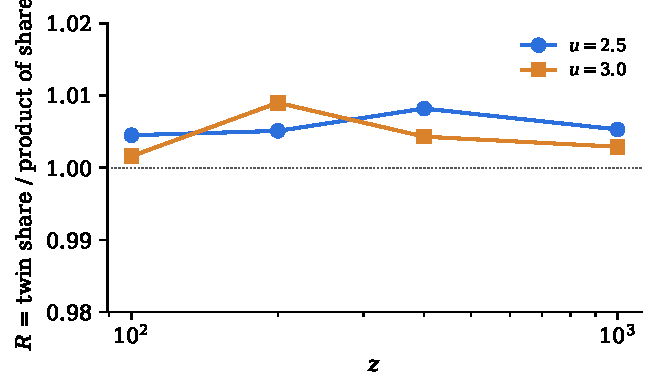
\includegraphics[width=0.52\linewidth]{fig6_frame.pdf}
\caption{The frame ratio $R$ of \cref{tab:frame}. The members of a rough pair are prime or not as two unbound numbers would be.}
\label{fig:frame}
\end{figure}

%======================================================================
\section{The principle and the twin law}\label{sec:law}

The construction contains one bond between the members of a pair, and \cref{thm:exclusion} proves that the bond is exclusion. Independence is not a further fact to be established. It is what remains when the relations have been listed.

\begin{principle}[independence is the absence of a relation]\label{pr:independence}
Two numbers are related only through a mechanism present in their construction. For the members $6k\pm1$ of a pair, the only mechanism is a clock, and a clock relates them only by exclusion (\cref{thm:exclusion}). A dependence between the members beyond exclusion, in any stretch of the integers, would be a relation without a clock.
\end{principle}

\begin{theorem}[the twin law]\label{thm:law}
Under \cref{pr:independence}, the number of twin prime pairs up to $x$ satisfies
\[
\pi_2(x)\sim\frac16\int_2^x\Bigl(\frac3{\log t}\Bigr)^2E\dd t=2C_2\int_2^x\frac{\dd t}{\log^2t}\sim\frac{2C_2\,x}{\log^2x},
\]
and there are infinitely many twin primes.
\end{theorem}
\begin{proof}
The centres up to $x$ number $x/6$. Among the numbers $\equiv\pm1\pmod 6$ near $t$, the primes have density $3/\log t$, because every prime above $3$ lies in these two classes, which hold a third of the integers. By \cref{thm:exclusion} and \cref{pr:independence}, the two members are prime as two unbound numbers, corrected at every clock by the exclusion factor, whose product is $E$. Summing over the centres gives the integral. Finally $\tfrac32E=2C_2$ by \cref{cor:constant}.
\end{proof}

The density $3/\log t$ and the constant $2C_2$ agree with the prediction of Hardy and Littlewood \cite{HL23}. In the present reading, that constant is nothing but the exclusion of the clocks.

\paragraph{The count.} \Cref{tab:law} and \cref{fig:law} compare the law with the count of twin pairs to $10^{10}$. From $10^7$ on, the count and the law agree to within $4$ parts in $10^3$. At $10^{10}$ they agree to $4.6$ parts in $10^5$.

\begin{table}[t]\centering\small
\begin{tabular}{@{}lrrr@{}}\toprule
$x$ & twin pairs $\le x$ & law $2C_2\int_2^x\dd t/\log^2t$ & ratio\\\midrule
$10^4$ & 205 & 214.2 & 0.9570\\
$10^5$ & 1{,}224 & 1{,}248.7 & 0.9802\\
$10^6$ & 8{,}169 & 8{,}248.0 & 0.9904\\
$10^7$ & 58{,}980 & 58{,}753.8 & 1.0039\\
$10^8$ & 440{,}312 & 440{,}367.8 & 0.99987\\
$10^9$ & 3{,}424{,}506 & 3{,}425{,}308.2 & 0.99977\\
$10^{10}$ & 27{,}412{,}679 & 27{,}411{,}416.5 & 1.00005\\\bottomrule
\end{tabular}
\caption{The twin law against the count of twin prime pairs.}
\label{tab:law}
\end{table}

\begin{figure}[t]\centering
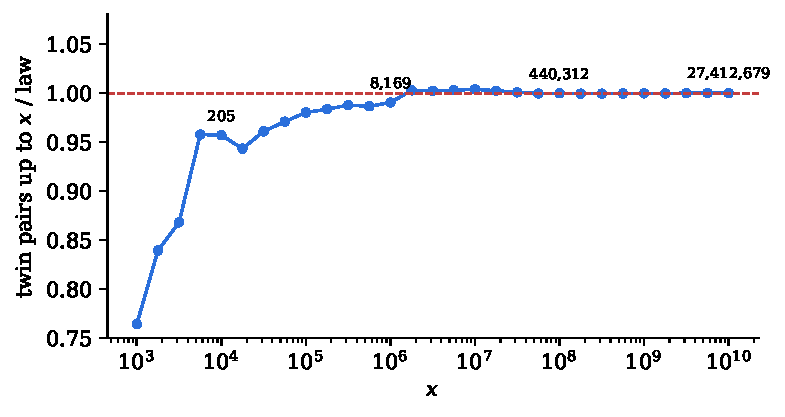
\includegraphics[width=0.7\linewidth]{fig5_law.pdf}
\caption{The count of twin pairs up to $x$ divided by the twin law, at quarter decades from $10^3$ to $10^{10}$.}
\label{fig:law}
\end{figure}

\paragraph{Where the burden lies.} In the convention of analytic number theory, carrying the exclusion law from the full turn of the clocks to the initial stretch $[1,x]$ is the content of the Hardy--Littlewood conjecture for twins, and is regarded as open. This paper asks instead what that transfer could fail by. A failure would be a correlation between $6k-1$ and $6k+1$ carried by no clock. It would have to show up somewhere, and we have looked for it in every place it could appear:
\begin{itemize}
\item per clock (\cref{thm:exclusion});
\item jointly over all clocks, in the full law of $(\Omega(6k-1),\Omega(6k+1))$;
\item in the pair symbol at every radius;
\item on the frame of rough pairs, after all small clocks have acted;
\item in the count to $10^{10}$.
\end{itemize}
The only departure from the product measured anywhere is the exclusion constant, to four decimals. The sign version of the principle, the independence of the parities $\lambda(n)$ and $\lambda(n+2)$ of the number of prime factors of neighbours, has been proved in logarithmic mean \cite{Tao16}. Gaps between primes are known to be bounded infinitely often \cite{Zhang14,Maynard15}.

%======================================================================
\section{The instrument and its ceiling}\label{sec:instrument}

This section proves that twins are forced by a majority, with no appeal to independence. It then measures exactly how much of that majority can be certified by information about the distribution of primes in residue classes, the information on which sieve methods rest \cite{FI}.

\begin{theorem}[twins by majority]\label{thm:pigeonhole}
Fix $z$ and $y$. Let $U$ be the number of rough pairs with $6k+1\le y$, and let $A$ and $B$ be the numbers of those whose lower, respectively upper, member is prime. Then the number of twin pairs among them is at least $A+B-U$. In particular, if more than half of the rough members on each side are prime, the range $(z,y]$ contains a twin pair.
\end{theorem}
\begin{proof}
For indicators, $[\text{lower prime}][\text{upper prime}]\ge[\text{lower prime}]+[\text{upper prime}]-1$ pointwise. Sum over the rough pairs.
\end{proof}

\begin{proposition}[the majority horizon]\label{prop:majority}
Among the numbers up to $y$ free of the primes up to $z=y^{1/u}$, the primes have share $1/(u\,\omega(u))$ asymptotically, where $\omega$ is Buchstab's function \cite{FI}. This share exceeds $\tfrac12$ exactly for $u<u^*$, with $u^*=3.565$.
\end{proposition}

On the frame of rough pairs the measured prime share of each member exceeds one half up to $u\approx3.8$ for $z$ between $30$ and $170$, and approaches $1/(u\,\omega(u))$ as $z$ grows (\cref{tab:majority,fig:instrument}). \Cref{thm:pigeonhole} then forces twins in every such range, with a guaranteed share of at least $2x-1$ of the frame, where $x$ is the prime share of each member.

\begin{table}[t]\centering\small
\begin{tabular}{@{}lcccc@{}}\toprule
 & $u=3.0$ & $u=3.5$ & $u=3.75$ & $u=4.0$\\\midrule
$z=30$: prime share / forced twins & 0.700 / 0.383 & 0.587 / 0.165 & 0.545 / 0.085 & 0.506 / 0.009\\
$z=60$ & 0.666 / 0.325 & 0.563 / 0.127 & 0.524 / 0.048 & 0.488 / --\\
$z=170$ & 0.645 / 0.289 & 0.548 / 0.097 & 0.510 / 0.019 & 0.476 / --\\
$z=1000$ & 0.624 / 0.247 & & & \\\bottomrule
\end{tabular}
\caption{Prime share of the members of rough pairs, and the share of twins it forces by \cref{thm:pigeonhole}. At $z=1000$, $u=3$ the forced share is $0.247$; the actual share is $0.390$.}
\label{tab:majority}
\end{table}

\begin{proposition}[the ceiling of the instrument]\label{prop:ceiling}
Suppose only the distribution of primes in residue classes is used, at the full level, and the frame count $U$ is known exactly. Then the largest share of rough members that can be certified prime is
\[
\max_u\ \frac1{u\,\omega(u)}\cdot\frac{f(u)}{\e^{\gamma}\omega(u)}=0.48837,\quad\text{attained at } u=3.16,
\]
where $f$ is the lower function of the linear sieve, which is optimal for this information \cite{FI}.

Allowing the two members different levels of roughness, the best certification of $A+B$ against $U$ is:
\begin{itemize}
\item $0.97881$ at level $\tfrac12$;
\item $0.98034$ at level $\tfrac47$;
\item $0.98058$ at level $\tfrac34$;
\item $0.99975$ at the full level.
\end{itemize}
The value $1$ is approached only as one member's roughness reaches the square root of the range. There that member is automatically prime, and \cref{thm:pigeonhole} reads twins $\ge$ twins.
\end{proposition}

\begin{figure}[t]\centering
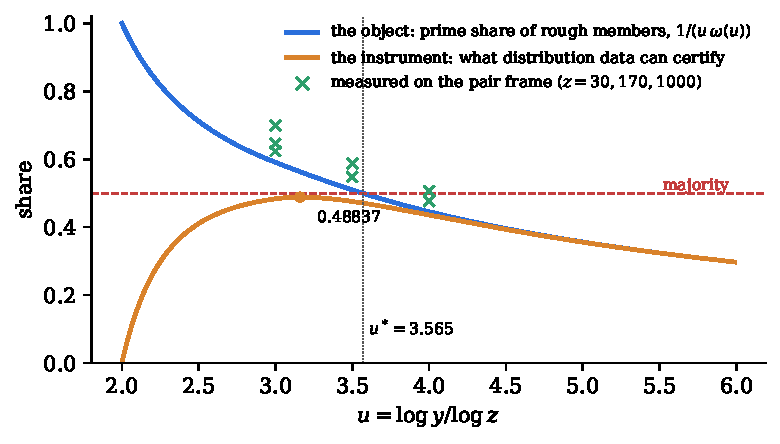
\includegraphics[width=0.8\linewidth]{fig7_instrument.pdf}
\caption{The object and the instrument. Blue: the prime share of rough numbers, above one half for $u<3.565$, where \cref{thm:pigeonhole} forces twins. Green: measured on the pair frame. Orange: the largest share that distribution information can certify, which never reaches one half (maximum $0.48837$).}
\label{fig:instrument}
\end{figure}

\paragraph{Reading.} A sieve sees only divisibility by small numbers. It cannot tell a prime from a product of two large primes, because both are free of small factors. \Cref{prop:ceiling} measures that blindness exactly. In the symmetric frame the instrument falls $1.16\%$ short of a majority. In the best asymmetric frame it closes the gap only where the inequality has become a tautology. Chen's method, which adds the switch of the two members, reaches a prime and a product of at most two primes \cite{Chen73} and stops at the same place. This is the parity barrier. It is a statement about what the instrument can see: the instrument cannot certify the majority that \cref{prop:majority} computes. It says nothing about whether the members of a pair are bound, which is the question of \cref{sec:exclusion,sec:measure}.

\paragraph{The reach as a frame.} The reach of the clocks (\cref{prop:mirror}) is a frame of rough pairs with $z=P$ and $y=P'^2$. So $u=2\log P'/\log P$, which tends to $2$. There \cref{thm:pigeonhole} becomes an equality. Buchstab's function at $u=2$ fixes the share of each member that the frame keeps against the turn.

\begin{proposition}[the frame at $u=2$]\label{prop:window}
Let $P<P'$ be consecutive primes with $P\ge5$. Take the centres of the reach, those with $6k-1>P$ and $6k+1<P'^2$. Let $n$ be their number, $U$ the number of rough pairs among them, and $A$ and $B$ the numbers of those whose lower, respectively upper, member is prime.
\begin{enumerate}[label=\textup{(\roman*)}]
\item $A=B=U$, and the number of twin pairs among these centres is exactly $A+B-U=U$.
\item The prime share $1/(u\,\omega(u))$ of \cref{prop:majority} equals $1$ for $1<u\le2$.
\item As $P\to\infty$,
\[
\frac{A}{n\prod_{5\le p\le P}(1-1/p)}\to\e^{\gamma}\omega(2)=\frac{\e^{\gamma}}2=0.89054,
\]
and the same holds for $B$.
\end{enumerate}
\end{proposition}
\begin{proof}
(i) By \cref{prop:mirror} a rough member of the reach is prime, so $A=U=B$. By \cref{thm:pigeonhole} the number of twin pairs is at least $A+B-U$, and it is at most $U$.
(ii) Buchstab's function satisfies $u\,\omega(u)=1$ for $1\le u\le2$ \cite{FI}.
(iii) The lower members are the primes $q\equiv5\pmod6$ with $P<q<P'^2-2$. By the prime number theorem for the progressions modulo $6$ \cite{Davenport}, $A\sim P'^2/(4\log P')$. Also $n\sim P'^2/6$, and by Mertens' theorem \cite{Mertens74} $\prod_{5\le p\le P}(1-1/p)=3\prod_{p\le P}(1-1/p)\sim3\e^{-\gamma}/\log P$. Since $P'<2P$, $\log P'/\log P\to1$, so the ratio tends to $\e^\gamma/2$. The upper members are the primes $q\equiv1\pmod6$ and have the same count.
\end{proof}

Over a full turn the share of full zeros is exactly $\prod_{5\le p\le P}(1-2/p)$, and the share of each member is $\prod(1-1/p)$ (\cref{thm:exclusion}). The reach is not a turn. By \cref{prop:window}(iii), each member keeps $\e^\gamma\omega(2)$ of its turn share there. In Buchstab's terms the turn share is the limit $u\to\infty$, where $\e^\gamma\omega(u)\to1$ \cite{FI}. Under \cref{pr:independence} the pair keeps the product of its members' factors. The twin law (\cref{thm:law}) at $x=P'^2$ gives
\[
U\sim\frac{2C_2P'^2}{\log^2(P'^2)}\sim\Bigl(\frac{\e^{\gamma}}2\Bigr)^2n\prod_{5\le p\le P}\Bigl(1-\frac2p\Bigr),\qquad \frac{\e^{2\gamma}}4=0.79305.
\]
\Cref{tab:window} measures the reach up to $P=31601$, where $P'^2>10^9$:
\begin{itemize}
\item The pair keeps the product of its members' factors to within $1.5\%$ for every $P\ge211$, and to within $0.3\%$ at $P=31601$.
\item The members keep $0.9387$ of their turn share. To within $0.04\%$, this is $\e^\gamma/2$ times $\pi(y)\log y/y=1.054$ at $y=P'^2$.
\item The pair keeps $0.8839$, and its factor falls with $P$ toward $0.7931$.
\end{itemize}

\begin{table}[t]\centering\small
\setlength{\tabcolsep}{4pt}
\begin{tabular}{@{}rrrrcccc@{}}\toprule
$P$ & centres $n$ & twins $U$ & turn share & $U$/turn share & lower & upper & pair/(lower$\cdot$upper)\\\midrule
$23$ & $135$ & $29$ & $28.87$ & $1.0044$ & $1.0415$ & $1.0113$ & $0.9537$\\
$101$ & $1{,}750$ & $208$ & $197.08$ & $1.0554$ & $1.0233$ & $1.0009$ & $1.0304$\\
$211$ & $8{,}252$ & $685$ & $699.47$ & $0.9793$ & $0.9919$ & $0.9841$ & $1.0034$\\
$503$ & $43{,}095$ & $2{,}631$ & $2{,}731.23$ & $0.9633$ & $0.9828$ & $0.9778$ & $1.0024$\\
$1009$ & $170{,}859$ & $8{,}332$ & $8{,}856.47$ & $0.9408$ & $0.9685$ & $0.9673$ & $1.0043$\\
$2003$ & $673{,}685$ & $27{,}075$ & $28{,}938.79$ & $0.9356$ & $0.9609$ & $0.9594$ & $1.0148$\\
$5003$ & $4{,}180{,}845$ & $130{,}803$ & $143{,}413.65$ & $0.9121$ & $0.9516$ & $0.9514$ & $1.0075$\\
$10007$ & $16{,}695{,}011$ & $440{,}825$ & $490{,}176.00$ & $0.8993$ & $0.9462$ & $0.9461$ & $1.0045$\\
$20011$ & $66{,}803{,}404$ & $1{,}510{,}202$ & $1{,}698{,}922.62$ & $0.8889$ & $0.9413$ & $0.9412$ & $1.0033$\\
$31601$ & $166{,}495{,}140$ & $3{,}420{,}966$ & $3{,}870{,}157.36$ & $0.8839$ & $0.9387$ & $0.9387$ & $1.0031$\\\midrule
limit & & & & $0.7931$ & $0.8905$ & $0.8905$ & $1$\\\bottomrule
\end{tabular}
\caption{The reach of the clocks up to $P$ as a frame at $u=2$: the centres with $6k-1>P$ and $6k+1<P'^2$. The turn share is $n\prod_{5\le p\le P}(1-2/p)$. Lower and upper: the prime members divided by $n\prod_{5\le p\le P}(1-1/p)$. The limits are $\e^{2\gamma}/4$ and $1$ under the twin law, and $\e^\gamma/2$ by \cref{prop:window}(iii).}
\label{tab:window}
\end{table}

\paragraph{What the frame at $u=2$ decides.} In the reach, \cref{thm:pigeonhole} reads twins $=U$. This is the degenerate case of \cref{prop:ceiling}, where the inequality has become twins $\ge$ twins, and it does not give the size of $U$. The count $U$ is the number of twin pairs between $P$ and $P'^2$. The share over a full turn, $n\prod_{5\le p\le P}(1-2/p)$, is not that count. In the reach each member keeps $\e^\gamma\omega(2)$ of its turn share, and at $P=31601$ the twin pairs number $0.884$ of the turn share. That $U>0$ for every $P$ means a twin pair between every prime and the square of the next. That is a statement about the twin primes themselves, and it implies that there are infinitely many. The reach is therefore the place where \cref{pr:independence} acts. The members' factors are theorems. That the pair keeps their product is the exclusion law carried from the turn into the reach.

%======================================================================
\section{Singles copy themselves; pairs never do}\label{sec:self-copy}

Let $\lambda$ be Liouville's function, the parity of the number of prime factors, and $L(x)=\sum_{n\le x}\lambda(n)$.

\begin{theorem}[a single is its own copy; a pair is not]\label{thm:copy}
\begin{enumerate}[label=\textup{(\roman*)}]
\item For every $x\ge1$, $\sum_{n\le x}\lambda(n)\lfloor x/n\rfloor=\lfloor\sqrt x\rfloor$.
\item For every even $D$ the equation $n(n+D)=m^2$ has finitely many solutions, all with $n<D^2/8+1$. Hence $\sum_{n\le x}\sum_{d\mid n(n+D)}\lambda(d)$ is bounded in $x$. For twins, $n(n+2)=(n+1)^2-1$ is never a square, and the sum is $0$ for every $x$.
\item For every $x\ge1$, $L(x)=\sum_{m\le x}\mu(m)\lfloor\sqrt{x/m}\rfloor$.
\end{enumerate}
\end{theorem}
\begin{proof}
(i) $\sum_{d\mid n}\lambda(d)$ is $1$ when $n$ is a square and $0$ otherwise; sum over $n\le x$. (ii) $(n+D/2-m)(n+D/2+m)=D^2/4$ has finitely many factorisations. (iii) is the Möbius inversion of (i).
\end{proof}

The sign-weighted count of single numbers is exactly the number of self-copies, the squares. That is the origin of the lean of the primes by one half. A pair's product is never its own copy, so a pair has no lean of its own: any lean of prime pairs must come from the copies of its members. Identity (iii) was checked exactly at eight values of $x$ up to $10^5$. Its first term, $\sqrt x\sum_{m\le x}\mu(m)m^{-1/2}$, is the source of the logarithmic mean of $L(x)/\sqrt x$, measured as $-0.682$ against $1/\zeta(\tfrac12)=-0.685$.

\begin{theorem}[the squares sit on the $+$ side]\label{thm:side}
Every prime $q\ge5$ has $q^2\equiv1\pmod{24}$, so $q^2$ lies on the $+$ side of the triad. For a pair $(n,n+D)$ of numbers prime to $6$:
\begin{itemize}
\item if $D\equiv2\pmod6$, only the upper member can be a prime square ($3\mid q^2+2$);
\item if $D\equiv4\pmod6$, only the lower member can be ($3\mid q^2-4$);
\item if $D\equiv0\pmod6$, both can be when $n\equiv1\pmod6$, and neither when $n\equiv5\pmod6$.
\end{itemize}
\end{theorem}

\begin{proposition}[the lean of a pair lives on its $+$ member]\label{prop:lean}
Suppose the pairs of prime powers $(n,n+D)$ are balanced over residue classes in the logarithmically weighted count. Then the class lean of prime pairs of gap $D\equiv2\pmod6$ is a function of the residue symbol of the upper member alone. The same holds for the lower member when $D\equiv4$, and for the pairs on the $+$ side when $D\equiv0$. The model in which a pair's lean is the product of its members' leans is incompatible with this for every modulus $q\ge5$.
\end{proposition}
\begin{proof}
This is the setting of the biases among prime pairs studied in \cite{LOS16}. Under the balance, prime pairs carry the negative of the prime-power pairs that contain a prime square. By \cref{thm:side}, for $D\equiv2$ these are $(q^2-D,q^2)$. Their centres $c$ have $c+D/2$ a nonzero square modulo $q$, and they are spread uniformly over those classes. The two symbols are linearly independent on the allowed classes for every $q\ge5$, which gives the incompatibility.
\end{proof}

\begin{figure}[t]\centering
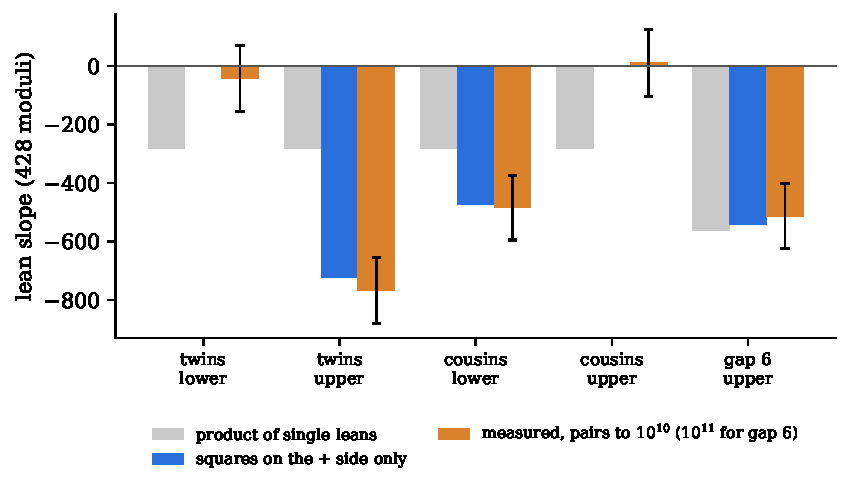
\includegraphics[width=0.8\linewidth]{fig9_lean.pdf}
\caption{Class lean of prime pairs over $428$ moduli $q\le3000$, per member. For twins the lower member carries no lean ($-42\pm112$ against $+3$) and the upper member carries it all ($-767\pm113$ against $-723$). Cousins show the same with the members exchanged. For gap $6$ the lower member keeps an excess of about $-190$ on both sides, about $2.5$ standard errors in combination.}
\label{fig:lean}
\end{figure}

\paragraph{The lean across $L$-functions.} For an $L$-function with normalised local sign $\lambda(p)$, under the generalised Riemann hypothesis the lean of the primes $\sum_{p\le x}\lambda(p)\log p/\sqrt p$ grows like $(-\nu/2-r)\log x$. Here $\nu$ is the slope of the self-copy sum $\sum\operatorname{tr}(\mathrm{Frob}_p^2)\log p/p$ and $r$ is the order of the zero at the centre. This is the form in which the rank enters the partial Euler products \cite{Goldfeld82,Conrad05,KimMurty23}, and the square term is the source of Chebyshev's bias \cite{RubinsteinSarnak94,SarnakLetter}. We measured both slopes separately, with primes to $10^9$, on $17$ objects (\cref{fig:selfcopy}):
\begin{itemize}
\item six complex characters, which have $\nu=0.000$ and no lean;
\item six real characters, the triad sign among them, with $\nu=0.999$ and lean $-0.49$ to $-0.50$;
\item two curves of rank $0$, with $\nu=-1.00$ and lean $+0.49$;
\item a curve of rank $1$, with lean $-0.48$ ($r=0.98$);
\item the symmetric squares, with $\nu=1.998$ with complex multiplication and $1.000$ without.
\end{itemize}
On the congruent-number curves the rank read from the lean, over $608$ curves, sorts into clusters with medians $1.00$ and $1.98$. These agree with Tunnell's criterion \cite{Tunnell83} and with the parity of the root number. The curve $n=210$ was read as rank $2$ from its primes before any point was known; a search then found two independent points, and three for $n=1254$.

\begin{figure}[t]\centering
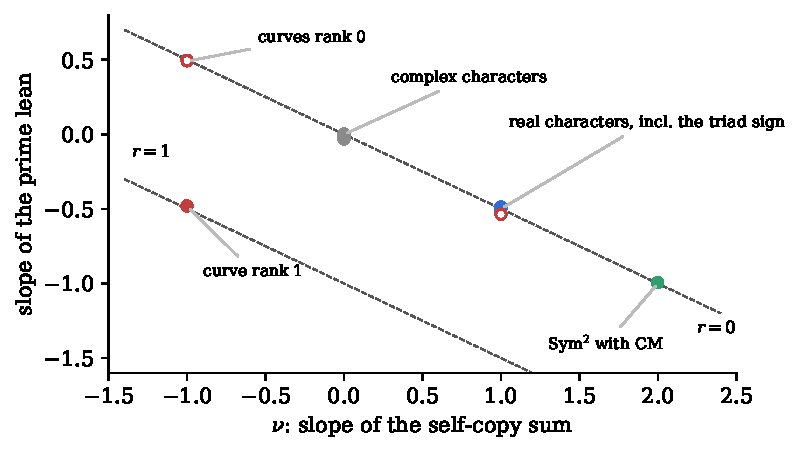
\includegraphics[width=0.68\linewidth]{fig10_selfcopy.pdf}
\caption{Lean of the primes against the self-copy count, for $17$ $L$-functions. All lie on the lines $-\nu/2-r$ with $r=0$ or $r=1$. Open circles: a curve without complex multiplication (level $11$) and its symmetric square.}
\label{fig:selfcopy}
\end{figure}

%======================================================================
\section{At the centre: the congruent-number curves}\label{sec:centre}

For squarefree $n$ let $E_n:y^2=x^3-n^2x$. Its coefficients follow from those of $E_1$ by the twist $a_p(E_n)=(\tfrac np)a_p(E_1)$. For $E_1$ itself, $a_p=0$ for $p\equiv3\pmod4$; otherwise write $p=a^2+b^2$ with $a$ odd, and then $a_p=\pm2a$, the sign $+$ exactly when $a+b\equiv1\pmod4$ \cite{Koblitz}. Tunnell's formula \cite{Tunnell83} expresses $L(E_n,1)\sqrt n$ as $\kappa_n(A-2B)^2$, where $A$ and $B$ count representations of $n$ by two ternary forms, with $\kappa_n=0.163879$ for odd $n$ and $0.327757$ for even $n$. We confirmed the formula on all $608$ squarefree $n\le1000$.

\begin{theorem}[the value at the centre is a square]\label{thm:square}
For squarefree $n$, $L(E_n,1)\sqrt n=4\kappa_n m^2$ with $m\in\Z$. Hence $L(E_n,1)$ is either $0$ or at least $4\kappa_n/\sqrt n$.
\end{theorem}
\begin{proof}
For odd $n$, every representation $x^2+2y^2+8z^2=n$ (and likewise for the second form) has $x$ odd, so the representations fall into sign classes of even size and $A$, $B$ are even; for even $n$ the same holds with $n/2$. Hence $A-2B=2m$.
\end{proof}

The value at the mirror point is a copy of a count, a square, and it cannot drift continuously to zero. Under the generalised Riemann hypothesis, Hadamard's product for the completed $L$-function, which is even about the centre, gives exactly $\sum_{\gamma>0}\gamma^{-2}=S_2/S_0$. Here $S_0$ and $S_2$ are rapidly converging sums over the coefficients, and $S_0$ carries the quantised central value. Hence $\gamma_1\ge(S_2/S_0)^{-1/2}$.

\Cref{tab:centre} shows one fact read five ways: a nearly balanced count, a small central value, a zero near the centre, a misread rank, and a slow Euler product.

\begin{table}[t]\centering\small
\begin{tabular}{@{}lcc@{}}\toprule
 & the $9$ curves read as rank $1.2$--$1.5$ & $12$ controls\\\midrule
Tunnell balance $|A-2B|$ & $4$ (smallest nonzero for $n>300$) & $24$--$36$\\
lowest zero above the centre $\gamma_1$ & $0.053$--$0.091$ & $0.323$--$0.537$\\
GRH floor $(S_2/S_0)^{-1/2}$, smallest of $247$ & $0.0375$ ($n=563$) & \\
Euler product at $10^9$ / limit & $0.38$, $0.50$ ($n=347,563$) & within $18\%$\\\bottomrule
\end{tabular}
\caption{The congruent-number curves $n=347,563,587,659,683,691,787,827,922$ against controls. A zero pair near the centre adds about $2\operatorname{sinc}(\gamma_1\log x)$ to the rank read from the primes. The Euler products of the controls column are those of $n=1,3,11,17,19,930$. The value $\gamma_1\approx0.05$--$0.1$ was predicted from the readings before the zeros were computed.}
\label{tab:centre}
\end{table}

\paragraph{The contrast with $\zeta$.} Take the finite pattern $\sum_{n\le N}n^{-s}$ with its mirror, cut at $N=\lfloor\sqrt{t/2\pi}\rfloor$. Its off-line pairs, found by complete scans of $10^3\le t\le10^5$ and of windows near $10^6$ and $10^7$, number $525$. The remainder of $\zeta$ closes every one of them back onto the line. All $525$ sit at heights where the prime clocks are anti-aligned: the sum $\sum_{p\le400}\cos(t\log p)/\sqrt p$ lies at a median percentile of $0.9\%$ among random heights. The closest of them, at $t=71732.91$, leaves $|Z|=0.00055$ between two zeros. For the congruent-number curves, \cref{thm:square} forbids a near-merge at the centre from becoming a merge except exactly. No such floor between neighbouring zeros is known for $\zeta$.

%======================================================================
\section{Which claims the step returns whole}\label{sec:whole}

A self-reproducing world proves its own persistence in one step: combined with a machine that runs it, the world produces the world again. The same test sorts the claims of this paper.

\paragraph{Returned whole by one step.}
\begin{itemize}
\item the count $\prod(p-2)$;
\item the palindrome;
\item the marking law and the copy sign;
\item the family of affine copies (\cref{thm:copies});
\item the exclusion law in the world of clocks (\cref{thm:exclusion});
\item the mirror symmetry of the zeros of $\xi$ as a set;
\item the twisting family of the congruent-number curves;
\item the square at the centre (\cref{thm:square}).
\end{itemize}

\paragraph{Not returned whole, and why.}
\begin{itemize}
\item \emph{Window claims about the reach} (\cref{sec:step}): the reach grows like $P^2$, the copies like $P$.
\item \emph{The statement that each zero of $\xi$ is its own mirror image}: the mirror alone returns only the set. Functions with the mirror but without the Euler product, such as Epstein zeta functions and the Davenport--Heilbronn function, have zeros off the line.
\item \emph{The pair $(m-1,m+1)$ under multiplication}: shift and multiplication do not commute. Seen from the centre, and modulo any prime, the pair is the unit pair $\pm1$, and every clock's marks are the square roots of $1$. Squaring respects both the mirror and multiplication, and in its terms a twin centre is a square $m^2$ whose predecessor $m^2-1$ splits into exactly two primes.
\end{itemize}

In every case the claim returns whole under the mirror or under multiplication. What is sought is the operation that is both. For the pair, \cref{thm:exclusion} shows that nothing beyond these two acts on it.

%======================================================================
\section{Methods}\label{sec:methods}
All computations are exact integer computations unless stated otherwise.
\begin{itemize}
\item \emph{Clock identities} (\cref{thm:count,thm:copies,thm:marking}) were checked by complete enumeration of turns for $P\le19$, and the window statistics over the full turn for $P=23$. The longest runs $H(P)$ come from exhaustive search over all rotations.
\item \emph{Twin counts} to $10^{10}$ come from a segmented sieve of Eratosthenes. The law was integrated numerically.
\item \emph{The joint law of $\Omega$} was computed for all $n\le3\cdot10^8$ by counting prime powers.
\item \emph{The rough frames} used a sieve to $10^9$, primality from the same sieve, and roughness by marking multiples of the primes up to $z$.
\item \emph{The reach as a frame} (\cref{tab:window}) used a sieve of the numbers $6k\pm1$ up to $10^9$ by the primes up to $31623$. Each clock marks its two classes, and $\pi(P'^2)=50{,}799{,}680$ at $P'=31607$.
\item \emph{The Buchstab function and the sieve functions $f$, $F$} were integrated from their delay equations with step $10^{-4}$. Checks: $\omega(3)=(1+\log2)/3$, $\omega(10)=\e^{-\gamma}$ to five digits, and $f(4)=0.97835$.
\item \emph{Class leans} were computed over $428$ prime moduli $q\le3000$ with the weight $\log^2m/\sqrt m$ at the centre $m$. Standard errors come from the spread of the per-modulus slopes.
\item \emph{The self-copy sums} used primes to $10^9$. The coefficients of the curve of level $11$ come from its eta product to $10^7$.
\item \emph{Central values} used the rapidly converging series, with the conductor ($32n^2$ for odd $n$, $16n^2$ for even $n$) confirmed by invariance in the cutoff parameter to $3\cdot10^{-14}$. The zeros are sign changes of the completed $L$-function on the line, by Gauss--Laguerre quadrature with $48$ nodes and step $0.002$. They are computed, not certified.
\end{itemize}

%======================================================================
\section{Concluding remarks}\label{sec:concl}
The paper set out to find what binds the two members of a twin pair. It found one thing. A clock can take one member, and in doing so it leaves the other. That bond is proved exactly, it fixes the twin constant, and every measurement of the pair shows it and nothing else. Read with the principle that independence is the absence of a relation, it gives the twin law and the recurrence of the twin pair at every level of the clocks. The one obstruction that has kept the question closed to the methods that know the most about primes is, on inspection, a limit of those methods' sight: they cannot tell one factor from two, and so they cannot certify the majority that the object itself carries. In the reach of the clocks the majority bound is an equality. There each member keeps $\e^\gamma/2$ of its turn share, and the twins keep the product of the two factors (\cref{prop:window}, \cref{tab:window}): this is the exclusion law carried into the reach.

\begin{thebibliography}{99}\small
\bibitem{Brun19} V.~Brun, La s\'erie $1/5+1/7+1/11+1/13+1/17+1/19+1/29+1/31+1/41+1/43+1/59+1/61+\cdots$, o\`u les d\'enominateurs sont ``nombres premiers jumeaux'' est convergente ou finie, \emph{Bull. Sci. Math.} 43 (1919) 100--104, 124--128.
\bibitem{Chen73} J.~R.~Chen, On the representation of a larger even integer as the sum of a prime and the product of at most two primes, \emph{Sci. Sinica} 16 (1973) 157--176.
\bibitem{Conrad05} K.~Conrad, Partial Euler products on the critical line, \emph{Canad. J. Math.} 57 (2005) 267--297.
\bibitem{Davenport} H.~Davenport, \emph{Multiplicative Number Theory}, 3rd ed., revised by H.~L.~Montgomery, Graduate Texts in Mathematics 74, Springer, New York, 2000.
\bibitem{DH08} H.~G.~Diamond, H.~Halberstam, \emph{A Higher-Dimensional Sieve Method}, with procedures for computing sieve functions by W.~F.~Galway, Cambridge Tracts in Mathematics 177, Cambridge University Press, 2008.
\bibitem{FGKMT} K.~Ford, B.~Green, S.~Konyagin, J.~Maynard, T.~Tao, Long gaps between primes, \emph{J. Amer. Math. Soc.} 31 (2018) 65--105.
\bibitem{FI} J.~Friedlander, H.~Iwaniec, \emph{Opera de Cribro}, American Mathematical Society Colloquium Publications 57, 2010.
\bibitem{Gallagher76} P.~X.~Gallagher, On the distribution of primes in short intervals, \emph{Mathematika} 23 (1976) 4--9.
\bibitem{Goldfeld82} D.~Goldfeld, Sur les produits partiels eul\'eriens attach\'es aux courbes elliptiques, \emph{C. R. Acad. Sci. Paris S\'er. I Math.} 294 (1982) 471--474.
\bibitem{HL23} G.~H.~Hardy, J.~E.~Littlewood, Some problems of `Partitio numerorum'; III: On the expression of a number as a sum of primes, \emph{Acta Math.} 44 (1923) 1--70.
\bibitem{Iwaniec78} H.~Iwaniec, On the problem of Jacobsthal, \emph{Demonstratio Math.} 11 (1978) 225--231.
\bibitem{KimMurty23} S.~Kim, M.~R.~Murty, From the Birch and Swinnerton-Dyer conjecture to Nagao's conjecture, \emph{Math. Comp.} 92 (2023) 385--408.
\bibitem{Koblitz} N.~Koblitz, \emph{Introduction to Elliptic Curves and Modular Forms}, 2nd ed., Graduate Texts in Mathematics 97, Springer, New York, 1993.
\bibitem{LOS16} R.~J.~Lemke Oliver, K.~Soundararajan, Unexpected biases in the distribution of consecutive primes, \emph{Proc. Natl. Acad. Sci. USA} 113 (2016) E4446--E4454.
\bibitem{Maynard15} J.~Maynard, Small gaps between primes, \emph{Ann. of Math.} 181 (2015) 383--413.
\bibitem{Mertens74} F.~Mertens, Ein Beitrag zur analytischen Zahlentheorie, \emph{J. Reine Angew. Math.} 78 (1874) 46--62.
\bibitem{MS04} H.~L.~Montgomery, K.~Soundararajan, Primes in short intervals, \emph{Comm. Math. Phys.} 252 (2004) 589--617.
\bibitem{RubinsteinSarnak94} M.~Rubinstein, P.~Sarnak, Chebyshev's bias, \emph{Experiment. Math.} 3 (1994) 173--197.
\bibitem{SarnakLetter} P.~Sarnak, Letter to B.~Mazur on Chebyshev's bias for $\tau(p)$, 2007, \url{https://publications.ias.edu/sites/default/files/MazurLtrMay08.PDF}.
\bibitem{Tao16} T.~Tao, The logarithmically averaged Chowla and Elliott conjectures for two-point correlations, \emph{Forum Math. Pi} 4 (2016) e8.
\bibitem{Tunnell83} J.~B.~Tunnell, A classical Diophantine problem and modular forms of weight $3/2$, \emph{Invent. Math.} 72 (1983) 323--334.
\bibitem{Zhang14} Y.~Zhang, Bounded gaps between primes, \emph{Ann. of Math.} 179 (2014) 1121--1174.
\end{thebibliography}
\end{document}
